\chapter{Matrix Theory Fundamentals}
\section{Determinant}

\noindent
The Determinant is a crucial number associated with square matrices, denoted either by $det(A)$ or $|A|$. A matrix $A$ is invertible iff (if and only if) $det(A) \neq 0$.

\noindent
Invertible matrix is called \textbf{non-singular.}
For a 2x2 matrix 
$
\begin{bmatrix}
a&b\\c&d
\end{bmatrix} $
the determinant is defined as 
$\begin{vmatrix}
a&b\\c&d
\end{vmatrix}$ $= ad-bc$.

\noindent

\begin{definitionbox}{Laplace's Formula for the Determinant} 
The determinant is defined as:

$det(\textbf{A}) = \sum^n_{j=1}(-1)^{i+j} a_{ij}M_{ij} $ for fixed i or \\
\noindent
$det(\textbf{A}) = \sum^n_{i=1}(-1)^{i+j} a_{ij}M_{ij} $ for fixed j 

This summation within can just be shortened to the produt of the cofactor and minor matrices within \textbf{A}, where:

\begin{itemize}
    \item The \emph{minor} \( M_{i,j} \) is defined to be the determinant of the \( (n - 1) \times (n - 1) \)-matrix that results from \( A \) by removing the \( i \)-th row and the \( j \)-th column.
    \item The \emph{cofactor} \( C_{i,j} \) is obtained by multiplying the minor by \( (-1)^{i+j} \).
\end{itemize}
\end{definitionbox}

\subsubsection*{Properties of Determinants}
\begin{enumerate}
    \item $det(I) = 1$ 
    \item Exchanging two rows of a matrix reverses the sign of the determinant. So an even number of exchanges keeps the determinant unchanged and an odd number of exchanges inverts the sign.
    \item Multiplying any row with a scalar multiplies the determinant by that scalar.
    \item Any row of zeroes leads to $det = 0$. \[
\begin{vmatrix}
0 & 0 \\
c & d
\end{vmatrix}
= 
\begin{vmatrix}
0 \cdot a & 0 \cdot b \\
c & d
\end{vmatrix}
=
0 \cdot
\begin{vmatrix}
a & b \\
c & d
\end{vmatrix}
= 0
\]
    \item Note that the determinant of the sum of two matrices is not necessarily the sum of their determinants:
\[
\begin{vmatrix}
a + a' & b + b' \\
c & d
\end{vmatrix} = \left(
\begin{vmatrix}
a  & b' \\
c & d
\end{vmatrix} + \begin{vmatrix}
a' & b' \\
c & d
\end{vmatrix} \right)
\neq
\begin{vmatrix}
a & b \\
c & d
\end{vmatrix}
+
\begin{vmatrix}
a' & b' \\
c & d
\end{vmatrix}
\]
In other words, \( \det(A + B) \neq \det(A) + \det(B) \). We observe `linearity' only for a single row
    \item Two equal rows leads to $det = 0$. This is inferred from the case of exchanging rows that changes the sign of the determinant – if we exchange two same rows, the final matrix is the same, so it should have the same sign – the only possible case of this is when $det=0$.
    \item Determinant after row reduction remains the same. \[
\begin{vmatrix}
a & b \\
c - la & d - lb
\end{vmatrix}
=
\begin{vmatrix}
a & b \\
c & d
\end{vmatrix}
+
\begin{vmatrix}
a & b \\
-la & -lb
\end{vmatrix}
=
\begin{vmatrix}
a & b \\
c & d
\end{vmatrix}
-
l
\begin{vmatrix}
a & b \\
a & b
\end{vmatrix}
=
\begin{vmatrix}
a & b \\
c & d
\end{vmatrix}
\]

\item Any upper or lower triangular matrix has the determinant that is the product of its diagonals.
\item Any singular matrix has $det = 0$ because eliminating the matrix gives it a row of zero. So this matrix is not full rank and is invertible. Any invertible matrix will have a non-zero determinant.
\item For square matrices $\textbf{A}$ and $\textbf{G}$ we have $det(\textbf{AB}) = det(\textbf{A})det(\textbf{B})$
    \item Moreover:
    \begin{itemize}
        \item The determinant of the inverse of \( A \) is the reciprocal of the determinant of \( A \):
        \[
        \det(A^{-1}) = \frac{1}{\det(A)}
        \]

        \item The determinant of \( A \) squared is the square of the determinant of \( A \):
        \[
        \det(A^2) = (\det(A))^2
        \]

        \item The determinant of a scalar multiple of \( A \) is the scalar raised to the \( n \)-th power times the determinant of \( A \), where \( A \) is an \( n \times n \) matrix and \( c \) is a scalar:
        \[
        \det(cA) = c^n\det(A)
        \]

    \end{itemize}

    \item The determinant of the transpose of \( A \) is equal to the determinant of \( A \):
    \[
    \det(A^T) = \det(A).
    \]
\end{enumerate}



\section{Rank and Trace}

\begin{definitionbox}{Rank of a matrix}
Given an \( m \times n \) matrix \( A \), the rank of \( A \), denoted \( \text{rank}(A) \), is the number of linearly independent rows or columns; in particular, if \( m = n \), \( \text{rank}(A) = n \) if and only if \( \det(A) \neq 0 \).

Properties (without proof):
\begin{itemize}
    \item For a rectangular matrix \( \text{rank}(A) \leq \min(n, m) \).
    \item \( \text{rank}(AB) \leq \min(\text{rank}(A), \text{rank}(B)) \).
\end{itemize}
\end{definitionbox}

\begin{definitionbox}{Trace of a matrix}
The trace of an \( n \times n \) matrix is defined as the sum of the elements along the main diagonal. Moreover:
\begin{itemize}
    \item \( \text{trace}(ABC) = \text{trace}(BCA) = \text{trace}(CAB) \).
    \item (Frobenius norm): \( \|A\|_F = \sqrt{\sum_{i,j} |a_{i,j}|^2} = \sqrt{\text{trace}(A^HA)} \) where \( A^H \) denotes the conjugate transpose of \( A \).
\end{itemize}
\end{definitionbox}


\section{Eigenvectors and Eigenvalues}
Consider a matrix \( A \) and a vector \( x \). The operation \( Ax \) produces a vector \( y \) at some direction. We are interested in vectors \( y \) which lie in the same direction as \( x \).\\    

In that case we have \( \textbf{Ax} = \lambda I \textbf{x} \) with \( \lambda \) being a scalar. Because the LHS is matrix multiplication and the RHS is scalar multiplication, we generally add in the identity matrix $I$ to help distinguish this:

\begin{align*}
    \textbf{Ax} &= \lambda I\textbf{x}\\
    (\textbf{A}-\lambda I)\textbf{x} &= 0
\end{align*}

 When the above relationship holds, \( x \) is called an \textit{eigenvector} and \( \lambda \) is called an \textit{eigenvalue} of matrix \( A \).\\

To solve this, if we know $(\textbf{A}-\lambda I)\textbf{x} = 0$, then $det((\textbf{A}-\lambda I)\textbf{x}) = 0$

If \( A \) is singular then \( \lambda = 0 \) is an eigenvalue.\\

Why are we interested in the eigenvectors and eigenvalues of a matrix? Because they make the solution of complex problems simpler. For example, if we know the eigenvectors and eigenvalues of a linear mapping \( y = Ax \) we can characterize that mapping easily.\\ If \( A = \begin{bmatrix} 3 & 1 \\ 1 & 3 \end{bmatrix} \), eigenvalues: \( \lambda_1 = 4 \), \( \lambda_2 = 2 \), eigenvectors: \( u_1 = \begin{bmatrix} 1 \\ 1 \end{bmatrix} \), \( u_2 = \begin{bmatrix} -1 \\ 1 \end{bmatrix} \).
Then \( x = a_1u_1 + a_2u_2 \) implies \( y = \lambda_1a_1u_1 + \lambda_2a_2u_2 \).

\begin{figure}[H]
    \centering
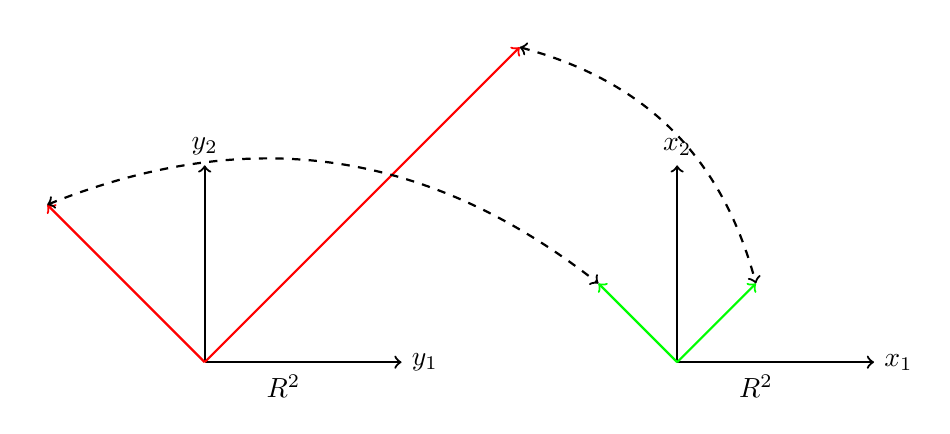
\begin{tikzpicture}[scale=1]

% Left plot (R^2 with y1, y2)
\begin{scope}[shift={(-3,0)}]
    % Axes
    \draw[thick,->] (0,0) -- (2.5,0) node[right] {$y_1$};
    \draw[thick,->] (0,0) -- (0,2.5) node[above] {$y_2$};
    % Vectors
    \draw[->, thick, red] (0,0) -- (4,4) node[above right] {};
    \draw[->, thick, red] (0,0) -- (-2,2) node[above left] {};
    % Label
    \node at (1,-0.3) {$\mathbb{R}^2$};
\end{scope}

% Right plot (R^2 with x1, x2)
\begin{scope}[shift={(3,0)}]
    % Axes
    \draw[thick,->] (0,0) -- (2.5,0) node[right] {$x_1$};
    \draw[thick,->] (0,0) -- (0,2.5) node[above] {$x_2$};
    % Vectors
    \draw[->, thick, green] (0,0) -- (1,1) node[above right] {};
    \draw[->, thick, green] (0,0) -- (-1,1) node[above left] {};
    % Label
    \node at (1,-0.3) {$\mathbb{R}^2$};
\end{scope}

% Curved double-ended arrows connecting corresponding vectors
% Connecting (4,4) in the left plot with (1,1) in the right plot
\draw[<->, thick, dashed] (-3+4,4) to[bend left] (3+1,1);
% Connecting (-2,2) in the left plot with (-1,1) in the right plot
\draw[<->, thick, dashed] (-3-2,2) to[bend left] (3-1,1);

\end{tikzpicture}

    \caption{Characterised mapping}
    \label{fig:eigens}
\end{figure}

In electrical engineering, we have already seen a few examples of this, for example, in continuous-time, such as the Signals and Systems module on eigen-functions of an LTI system leading to the convolution formula in the Fourier domain, and the solutions of linear differential equations in Control Systems.\\

In the discrete-time finite dimensional case, eigenvalues and eigenvectors are very important for discrete-time convolution and for difference equations.\\

\subsection{Eigenvectors and Eigenvalues of a permutation matrix}

Consider permutation matrix $\textbf{A} = \begin{bmatrix}
    0 & 1 \\ 1 & 0
\end{bmatrix}$.

It will have eigenvector $\begin{bmatrix}
    1\\1
\end{bmatrix}$ with corresponding eigenvalue $\lambda = 1$, and eigenvector $\begin{bmatrix}
    -1\\1
\end{bmatrix}$ with corresponding eigenvalue $\lambda = -1$.

Note that $n\times n$ matrices will have $n$ eigenvalues, but it is not easy to find them. In this syllabus, we do not go into much detail about the properties of eigenvalues and eigenvectors of a permutation matrix, but we can say that since permutation matrices are orthogonal, the eigenvectors span an orthogonal basis.\\

\subsubsection*{Properties}
\begin{itemize}
    \item The sum of eigenvalues, the \textbf{trace} of the matrix, equals the sum of the diagonal elements of the matrix.
    \item The product of eigenvalues equals the determinant of the matrix.
    \item We could have worked out the second eigenvalue of \textbf{A} by simply dividing the determinant by the first eigenvalue
\end{itemize}

\subsection{Solving for Eigenvalues and Eigenvectors}
\begin{definitionbox}{Finding Eigenvalues}
The eigenvalues of a matrix $A$ are found by solving the characteristic equation:
\[
\det(A - \lambda I) = 0
\]
where $I$ is the identity matrix of the same size as $A$.
\end{definitionbox}

\begin{definitionbox}{Finding Eigenvectors}
Once the eigenvalues $\lambda_i$ are found, the corresponding eigenvectors $v_i$ are found by solving the system of linear equations given by:
\[
(A - \lambda_i I)v_i = 0
\]
This system is solved for each eigenvalue $\lambda_i$. Note that there exists families of eigenvectors, not single eigenvectors.
\end{definitionbox}

\subsubsection*{Example}
For matrix $A = \begin{pmatrix}
2 & 1 \\
1 & 2
\end{pmatrix}$, we find eigenvalues by solving $\det(A - \lambda I) = 0$:

\[
\begin{vmatrix}
2 - \lambda & 1 \\
1 & 2 - \lambda
\end{vmatrix} = (2-\lambda)^2 - 1 = \lambda^2 - 4\lambda + 3 = 0
\]

This gives $\lambda_1 = 1$ and $\lambda_2 = 3$. The eigenvectors are found by substituting $\lambda_i$ back into $(A - \lambda_i I)v_i = 0$.

\subsubsection*{Example}
Consider the matrix 
\[ A = \begin{bmatrix}
3 & 1 \\
0 & 3
\end{bmatrix}. \]

The sum of the eigenvalues \( \lambda_1 + \lambda_2 \) is equal to the trace of \( A \), which is 6, and the product \( \lambda_1 \lambda_2 \) is equal to the determinant of \( A \), which is 9.

To find the eigenvalues, we calculate the determinant of \( A - \lambda I \):
\[ \det(A - \lambda I) = \det \begin{bmatrix}
3 - \lambda & 1 \\
0 & 3 - \lambda
\end{bmatrix} = (3 - \lambda)^2 = 0 \Rightarrow \lambda_{1,2} = 3. \]

\textbf{The eigenvalues of a triangular matrix are the values of the diagonal.}

For this particular case, we have:
\[ \begin{bmatrix}
3 & 1 \\
0 & 3
\end{bmatrix}
\begin{bmatrix}
x \\
y
\end{bmatrix}
=
\begin{bmatrix}
3x \\
3y
\end{bmatrix}
\Rightarrow y = 0 \text{ and } x \text{ can be any number.}
\]
\subsection{Special Case: Eigenvalues with Identity Matrix Addition}
Consider the matrix $\textbf{A} = \textbf{B} + c\textbf{I}$.\\

Consider an eigenvector \textbf{x} and eigenvalue $\lambda$ of \textbf{B}.\\

Then \textbf{Bx} = $\lambda\textbf{x}$ and so:\\

\begin{align*}
    \textbf{Ax} &= (\textbf{B} + c\textbf{I})\textbf{x}\\
    &= \textbf{Bx} + c\textbf{Ix}\\
    &= \textbf{Bx} + c\textbf{x}\\
    &= \lambda\textbf{x} + c\textbf{x}\\
    &= (\lambda+ c)\textbf{x}
\end{align*}

From this we can say \textbf{A} has the same eigenvectors as \textbf{B} with eigenvalues $\lambda + c$.
% \subsubsection*{Properties}


\section{Diagonalisation of Matrices}
\begin{itemize}
    \item Suppose we have \( n \) linearly independent eigenvectors of a matrix \( A \), denoted by \( \mathbf{x}_i \).
    \item The corresponding eigenvalues are \( \lambda_i \).
    \item These eigenvectors are arranged as columns in a matrix \( S \), forming the so-called eigenvector matrix.
    \item By forming the product \( AS \), where \( S = [\mathbf{x}_1 \mathbf{x}_2 \ldots \mathbf{x}_n] \), we effectively scale each eigenvector by its corresponding eigenvalue:
    \[
    AS = A[\mathbf{x}_1 \mathbf{x}_2 \ldots \mathbf{x}_n] = [\lambda_1\mathbf{x}_1 \lambda_2\mathbf{x}_2 \ldots \lambda_n\mathbf{x}_n] = S\Lambda
    \]
    where \( \Lambda \) is a diagonal matrix with eigenvalues \( \lambda_i \) on its diagonal and zeros elsewhere:
    \[
    \Lambda = \begin{bmatrix}
    \lambda_1 & 0 & \ldots & 0 \\
    0 & \lambda_2 & \ldots & 0 \\
    \vdots & \vdots & \ddots & \vdots \\
    0 & 0 & \ldots & \lambda_n
    \end{bmatrix}
    \]
    \item This gives us the fundamental relationship \( AS = S\Lambda \), which implies \( A = S\Lambda S^{-1} \) when \( S \) is invertible.
    \item The process of transforming \( A \) into \( \Lambda \) through the similarity transformation \( S \) is called \emph{matrix diagonalisation}.
    \item Matrix diagonalisation is particularly important in Mathematics and Engineering because it simplifies many matrix computations and provides a clear framework for understanding linear transformations.
\end{itemize}

\subsection{Matrix Diagonalisation and Commutativity}

\textbf{Theorem:} Matrices \( A \) and \( B \) are simultaneously diagonalisable, sharing the same eigenvector matrix \( S \), if and only if \( AB = BA \).\\

\textit{Sketch of the proof:} Given that \( A \) and \( B \) are diagonalisable, we can write \( A = S\Lambda_1S^{-1} \) and \( B = S\Lambda_2S^{-1} \). Thus, 
\[ AB = S\Lambda_1S^{-1}S\Lambda_2S^{-1} \] 
and 
\[ BA = S\Lambda_2S^{-1}S\Lambda_1S^{-1} \].
Since \( \Lambda_1\Lambda_2 = \Lambda_2\Lambda_1 \) (as they are diagonal matrices), it follows that \( AB = BA \).\\

A matrix has \( n \) independent eigenvectors and therefore is diagonalisable if all the eigenvalues are different.\\

If \( Ax = \lambda x \) then \( A^2x = A(Ax) = A(\lambda x) = \lambda (Ax) = \lambda^2 x \). Therefore, the eigenvalues of \( A^2 \) are \( \lambda^2 \). The eigenvectors of \( A^2 \) remain the same since \( A^2 = SAS^{-1}SAS^{-1} = S\Lambda^2S^{-1} \). In general, for any positive integer \( k \), \( A^k = S\Lambda^kS^{-1} \).\\

If there are repeated eigenvalues a matrix may, or may not have independent eigenvectors. For example, consider the identity matrix. Its eigenvectors are the row (or column) vectors. They are all independent, but the eigenvalues are all equal to 1.\\
 \begin{examplebox}{A and B sharing Eigenvectors}
\subsubsection*{Question}
If \( A \) and \( B \) share the same eigenvectors, what can we say about the eigenvalues of \( AB \)?

\subsubsection*{Answer} Since $A$ and $B$ share the same eigenvectors, $AB$ will also have the same eigenvectors. Let $v$ be an eigenvector of $A$ and $B$, then $Av = \lambda v$ and $Bv = \mu v$ for some eigenvalues $\lambda$ and $\mu$ of $A$ and $B$ respectively. Thus:

\[ABv = A(\mu v) = \mu Av = \mu\lambda v\]

Showing us that $v$ is also an eigenvector of $AB$ with corresponding eigenvalue $\mu\lambda$. But this does not tell us that all eigenvalues of $AB$ are necessarily products of eigenvalues of $A$ and $B$. $A$ and $B$ must be diagonalisable and $A,B$ are commutative so $AB = BA$. $A=PDP^{-1}$ and $B = PQP^{-1}$, where $D$ and $Q$ are diagonal matrices with eigenvalues of $A$ and $B$ respectively, and $P$ is the matrix of shared eigenvectors. Then $AB = PDQP^{-1}$, and the eigenvectors form a basis, so diagonal entries of $DQ$ will be eigenvalues of $AB$ since the determinant between the two are preserved. \\
\end{examplebox}

\begin{examplebox}{Inverting a Diagonalisable Square Matrix}    

\subsubsection*{Question} If \( A = S\Lambda S^{-1} \) is square and invertible, can you compute \( A^{-1} \)?

\subsubsection*{Answer} If \( A \) is invertible, then \( A^{-1} = S\Lambda^{-1}S^{-1} \), where \( \Lambda^{-1} \) is the diagonal matrix with the reciprocal of \( A \)'s eigenvalues on the diagonal.
\end{examplebox}


\section{Difference Equations}
\subsection*{Fibonacci Sequence Analysis}

The Fibonacci sequence (0,1,1,2,3,5,8,13...) is a series of numbers where each number is the sum of the two preceding ones, typically starting with 0 and 1. Mathematically, it can be expressed as:
\begin{equation}
    F_{k+2} = F_{k+1} + F_k
\end{equation}
where $F_k$ represents the $k$-th term of the Fibonacci sequence.

To solve this using linear algebra, we can define the state vector $u_k$:
\begin{equation}
    u_k = \begin{bmatrix}
    F_{k+1} \\
    F_k
    \end{bmatrix}
\end{equation}
By employing the recursive definition of the Fibonacci sequence, we obtain the matrix form:
\begin{equation}
    u_{k+1} = A u_k = \begin{bmatrix}
    1 & 1 \\
    1 & 0
    \end{bmatrix} u_k
\end{equation}
Given the initial state vector $u_0$ that we know of, the state at any point $k$ is given by:
\begin{equation}
    u_k = A^k u_0
\end{equation}
If $A$ can be diagonalized as $A = S \Lambda S^{-1}$, where $\Lambda$ is a diagonal matrix of eigenvalues and $S$ is a matrix of corresponding eigenvectors, then the computation simplifies to:
\begin{equation}
    u_k = S \Lambda^k S^{-1} u_0
\end{equation}
Thus, knowing the eigenvectors and eigenvalues of $A$ can greatly simplify the computation of terms in the Fibonacci sequence.

\subsection*{System of Difference Equations}

Consider a system described by a set of difference equations:
\begin{align}
    y_1[n+1] &= y_1[n] - 1.5y_2[n] \\
    y_2[n+1] &= 0.5y_1[n] + y_2[n]
\end{align}
This system can be written in matrix form using the state vector $u_n$:
\begin{equation}
    u_n = \begin{bmatrix}
    y_1[n] \\
    y_2[n]
    \end{bmatrix}
\end{equation}
Thus, the next state $u_{n+1}$ is given by:
\begin{equation}
    u_{n+1} = A u_n = \begin{bmatrix}
    1 & -1.5 \\
    0.5 & 1
    \end{bmatrix} u_n
\end{equation}
Given $u_0$, the state $u_n$ is then:
\begin{equation}
    u_n = A^n u_0
\end{equation}
As with the Fibonacci sequence, if $A$ can be diagonalized, the solution becomes more tractable:
\begin{equation}
    u_n = S \Lambda^n S^{-1} u_0
\end{equation}
Hence, eigenvalues and eigenvectors are key to simplifying the solution of the system of difference equations, providing a powerful method to analyze and solve linear discrete-time systems in signals and systems.\\

\section{Markov Processes}
Markov processes are used to model systems that undergo transitions from one state to another on a state space. A key feature of a Markov process is that the future state depends only on the current state and not on the sequence of events that preceded it.\\


Consider a Markov process example inspired by Strang's book, modelling population migration between California and the outside:
\begin{quote}
    ``Assume that each year 1/10 of the people outside California move in and 2/10 of the people inside California move out."
\end{quote}

Let $y_0$ be the initial population outside California and $z_0$ the initial population inside California. The state vector and the transition matrix $A$ are given by:
\begin{equation}
    \begin{bmatrix}
    y_1 \\
    z_1 
    \end{bmatrix} = 
    \begin{bmatrix}
    0.9 & 0.2 \\
    0.1 & 0.8 
    \end{bmatrix}
    \begin{bmatrix}
    y_0 \\
    z_0 
    \end{bmatrix} = A 
    \begin{bmatrix}
    y_0 \\
    z_0 
    \end{bmatrix}
\end{equation}


The eigenvalues and eigenvectors of $A$ are crucial for understanding the long-term behavior of the Markov process. In this case, the eigenvalues are $\lambda_1 = 1$ and $\lambda_2 = 0.7$, with corresponding eigenvectors:
\begin{equation}
    \mu_1 = \begin{bmatrix}
    2/3 \\
    1/3 
    \end{bmatrix}, \quad
    \mu_2 = \begin{bmatrix}
    1 \\
    -1 
    \end{bmatrix}
\end{equation}
We can then write the state at instant $k$ as:
\begin{equation}
    \begin{bmatrix}
    y_k \\
    z_k 
    \end{bmatrix} = A^k
    \begin{bmatrix}
    y_0 \\
    z_0 
    \end{bmatrix}
\end{equation}

For a large $k$, the contribution from the second eigenvalue becomes negligible, leading to a steady-state solution where the population distribution does not change from one year to the next:
\begin{equation}
    \begin{bmatrix}
    y_{\infty} \\
    z_{\infty} 
    \end{bmatrix} = \left( y_0 + z_0 \right)
    \begin{bmatrix}
    2/3 \\
    1/3 
    \end{bmatrix}
\end{equation}

\subsection*{Properties of Transition Matrices}

From this example, we can deduce some general properties of Markov or transition matrices:
\begin{itemize}
    \item All entries are non-negative.
    \item Each column of the matrix adds up to one, ensuring the total probability is conserved.
    \item The eigenvalue $\lambda_1 = 1$ corresponds to the steady state.
    \item All other eigenvalues $\lambda_i$ satisfy $|\lambda_i| \leq 1$.
\end{itemize}
Additionally, it can be shown that $\lambda_1 = 1$ is always an eigenvalue by noting that each column of $A - I$ sums to zero, indicating that $A - I$ is singular and thus $\lambda_1 = 1$ is an eigenvalue. The corresponding eigenvector represents the steady-state distribution since $A\mu_1 = \mu_1$. This implies that in the long run, the system will reach a state where the population distribution remains constant if no external changes are made to the system.

\subsection*{Computing the State at Instant \( k \)}

Given the eigendecomposition of \( A \) as \( A = S \Lambda S^{-1} \), where \( S \) is the matrix of eigenvectors and \( \Lambda \) is the diagonal matrix of eigenvalues, the state at any instant \( k \) can be computed as:
\begin{equation}
    \begin{bmatrix}
    y_k \\
    z_k 
    \end{bmatrix} = S \Lambda^k S^{-1}
    \begin{bmatrix}
    y_0 \\
    z_0 
    \end{bmatrix}
\end{equation}

For our specific matrix \( A \), the computation yields:
\begin{equation}
    \begin{bmatrix}
    y_k \\
    z_k 
    \end{bmatrix} = 
    \begin{bmatrix}
    2/3 & 1/3 \\
    1/3 & -1/3 
    \end{bmatrix}
    \begin{bmatrix}
    1 & 0 \\
    0 & (0.7)^k 
    \end{bmatrix}
    \begin{bmatrix}
    1 & 1 \\
    1 & -2 
    \end{bmatrix}
    \begin{bmatrix}
    y_0 \\
    z_0 
    \end{bmatrix}
\end{equation}

\subsection*{Steady-State Solution}

The steady-state solution, which occurs as \( k \) approaches infinity, is given by the eigenvector corresponding to \( \lambda_1 = 1 \):
\begin{equation}
    \begin{bmatrix}
    y_{\infty} \\
    z_{\infty} 
    \end{bmatrix} = 
    \left( y_0 + z_0 \right)
    \begin{bmatrix}
    2/3 \\
    1/3 
    \end{bmatrix}
\end{equation}
This indicates that regardless of the initial state, the system will evolve into a state where the ratios of the populations inside and outside California are \( 2:1 \), respectively.

\subsection*{General Observations}

The model demonstrates a fundamental principle of Markov processes: despite potentially complex dynamics, the long-term behaviour is determined by the eigenvalues and eigenvectors of the transition matrix, with the largest eigenvalue indicating the steady state. This simplifies the analysis of systems described by Markov processes, particularly in the fields of signals and systems, stochastic processes, and population dynamics.



\section{Diagonalisation of Circulant Matrices}

Diagonalization of circulant matrices is closely tied to the concept of convolution in signal processing. A circulant matrix \( A \) can model the circular convolution operation between an input vector \( \mathbf{x} \) and a filter \( \mathbf{h} \), resulting in an output vector \( \mathbf{y} \) such that \( \mathbf{y} = A\mathbf{x} \).

\subsubsection*{Discrete Fourier Transform (DFT)}

The Discrete Fourier Transform (DFT) plays a pivotal role in the analysis of circulant matrices. For a DFT matrix of size \( n \times n \), the element in the \( i \)-th row and \( k \)-th column is given by \( w_n^{ik} \), where \( w_n = e^{-j\frac{2\pi}{n}} \). The DFT matrix \( W \) has the following form:

\[
W = \frac{1}{\sqrt{n}} \begin{bmatrix} 
1 & 1 & 1 & \cdots & 1 \\
1 & w_n & w_n^2 & \cdots & w_n^{n-1} \\
1 & w_n^2 & w_n^4 & \cdots & w_n^{2(n-1)} \\
\vdots & \vdots & \vdots & \ddots & \vdots \\
1 & w_n^{n-1} & w_n^{2(n-1)} & \cdots & w_n^{(n-1)(n-1)}
\end{bmatrix}
\]

\subsubsection*{Eigenvectors and Eigenvalues}

The eigenvectors of a circulant matrix are precisely the columns of the DFT matrix \( W \). These eigenvectors, denoted as \( \mathbf{u}_i \), can be expressed as:

\[
\mathbf{u}_i = \frac{1}{\sqrt{n}} \begin{bmatrix}
1 \\
w_n^i \\
w_n^{2i} \\
\vdots \\
w_n^{(n-1)i}
\end{bmatrix}
\]

The eigenvalues of a circulant matrix are the DFT of the first row of the matrix, which corresponds to the filter \( \mathbf{h} \). This direct correspondence facilitates the use of DFT in signal processing to perform efficient convolution operations.

\subsubsection*{Diagonalization by DFT}

The DFT matrix \( W \) has the property of diagonalizing a circulant matrix \( A \). This means that \( A \) can be represented as \( A = W \Lambda W^{-1} \), where \( \Lambda \) is a diagonal matrix containing the eigenvalues of \( A \). As a result, the DFT simplifies the multiplication of a circulant matrix with a vector, transforming it into a multiplication of the diagonal matrix \( \Lambda \) with the DFT of the vector.

\subsubsection*{Implications in Signal Processing}

In signal processing, this diagonalization property is exploited for efficient computation of convolutions, particularly using algorithms such as the Fast Fourier Transform (FFT), which is a computationally efficient implementation of the DFT. Thus, the DFT forms the basis for many signal processing techniques, enabling the analysis and manipulation of signals in the frequency domain.

\section{Complex, Symmetric, Hermitian Matrices}

Symmetric matrices are a fundamental concept in linear algebra with important implications in various fields, including signal processing and systems theory. 

\subsection*{Definition and Properties}

\begin{itemize}
    \item A real matrix \( A \) is said to be symmetric if \( A = A^T \), where \( A^T \) denotes the transpose of \( A \).
    \item For complex matrices, symmetry is defined by the condition \( A^* = A \), where \( A^* \) denotes the conjugate transpose of \( A \). Such matrices are also known as \textit{Hermitian matrices}.
    \item The notation \( A^H \) is also commonly used to denote the conjugate transpose, so for Hermitian matrices, \( A^H = A \).
    \item Symmetric matrices are prevalent in numerous applications, notably in statistics as covariance matrices.
    \item It is an established fact that the eigenvalues of a symmetric matrix are real numbers. This will be demonstrated through a proof.
    \item Additionally, eigenvectors of a symmetric matrix corresponding to distinct eigenvalues are orthogonal. The proof of this statement is provided in a subsequent section.
    \item For symmetric matrices with orthonormal eigenvectors, we can represent \( A \) as \( A = Q\Lambda Q^T \), where \( Q \) is the matrix of eigenvectors, and \( \Lambda \) is the diagonal matrix of eigenvalues.
\end{itemize}

\subsection*{Eigenvalues and Eigenvectors}
\begin{examplebox}{Proof of Complex Conjugate Pairs for Eigenvalues}
\subsubsection*{Question}

Prove that the eigenvalues of a symmetric matrix occur in complex conjugate pairs.

\subsubsection*{Solution}

Consider the eigenvalue equation \( Ax = \lambda x \).

\begin{itemize}
    \item Taking the complex conjugate of both sides of the equation yields \( (Ax)^* = (\lambda x)^* \) which simplifies to \( A^* x^* = \lambda^* x^* \).
    \item If \( A \) is a real symmetric matrix, then \( A^* = A \), and hence \( \lambda^* x^* \) must also be an eigenvector-eigenvalue pair, i.e., if \( \lambda \) is an eigenvalue of \( A \) with corresponding eigenvector \( x \), then \( \lambda^* \) is also an eigenvalue of \( A \) with corresponding eigenvector \( x^* \).
\end{itemize}

\end{examplebox}

\begin{examplebox}{Proof that Symmetric Matrices' Eigenvalues are Real}
\subsubsection*{Question}
Prove that the eigenvalues of a symmetric matrix are real.

\subsubsection*{Solution}

We have previously shown that for a real matrix \( A \), the complex conjugate of an eigenvalue \( \lambda \) is also an eigenvalue. Let's consider the eigenvalue equation \( Ax = \lambda x \).

\begin{enumerate}
    \item Taking the transpose of both sides of the equation yields \( x^T A^T = \lambda x^T \). Since \( A \) is symmetric, \( A^T = A \), so this becomes \( x^T A = \lambda x^T \).
    \item Multiplying both sides from the right by \( x \), we get \( x^T Ax = \lambda x^T x \).
    \item Now, we take the eigenvalue equation \( Ax = \lambda x \) and multiply both sides from the left with \( x^T \) to obtain \( x^T Ax = \lambda x^T x \).
    \item Observing the above, since \( x^T x \) is a scalar and \( x^T x \neq 0 \), it implies that \( \lambda \) must be equal to its complex conjugate \( \lambda^* \), which means \( \lambda \) is real.
\end{enumerate}
  
\end{examplebox}
\begin{examplebox}{Proof that Eigenvectors of a Symmetric Matrix with Unique Eigenvalues are always Orthogonal}
\subsubsection*{Question}
Prove that the eigenvectors of a symmetric matrix corresponding to different eigenvalues are always orthogonal.

\subsubsection*{Solution}

Let \( Ax = \lambda_1 x \) and \( Ay = \lambda_2 y \) be two eigenvectors of \( A \) corresponding to distinct eigenvalues \( \lambda_1 \neq \lambda_2 \).

\begin{enumerate}
    \item Taking the dot product of \( Ax \) with \( y \) yields \( (Ax)^T y = \lambda_1 x^T y \).
    \item Since \( A \) is symmetric, \( (Ax)^T y = x^T A^T y = x^T Ay = x^T \lambda_2 y \).
    \item These conditions imply \( \lambda_1 x^T y = \lambda_2 x^T y \) and since \( \lambda_1 \neq \lambda_2 \), it follows that \( x^T y = 0 \).
    \item Thus, the eigenvectors \( x \) and \( y \) are orthogonal.
\end{enumerate}



\end{examplebox}




\begin{definitionbox}{A Hermitian Matrix always has Real Eigenvectors}
\begin{itemize}
    \item We aim to determine which complex matrices have real eigenvalues and orthogonal eigenvectors.
    \item Consider the eigenvalue equation \( Ax = \lambda x \) with \( A \) possibly complex.
    \item Taking the complex conjugate on both sides yields \( (Ax)^* = (\lambda x)^* \) which implies \( A^* x^* = \lambda^* x^* \).
    \item By transposing both sides, we obtain \( x^{*T} A^{*T} = \lambda^* x^T \).
    \item Multiplying both sides from the right by \( x \), we get \( x^* A^* x = \lambda^* x^T x \).
    \item Starting again with \( Ax = \lambda x \) and multiplying both sides from the left by \( x^* \), we have \( x^* Ax = \lambda x^* x \).
\end{itemize}
    From the above steps, we deduce that if \( A^{*T} = A \), then \( \lambda x^* x = \lambda^* x^* x \) and since \( x^* x \neq 0 \), it follows that \( \lambda = \lambda^* \).
\end{definitionbox}

\begin{examplebox}{Proof of Orthogonal Eigenvectors for unique Eigenvectors in Hermitian Matrices\\ }
\subsubsection*{Question:}
Prove that the eigenvectors of a complex symmetric matrix (Hermitian matrix) which correspond to different eigenvalues are always perpendicular.

\subsubsection*{Solution:}
Suppose $Ax = \lambda_1 x$ and $Ay = \lambda_2 y$,where $\lambda_1 \neq \lambda_2$. We have

\[(\lambda_1x)^Hy=x^H\lambda_1y=(Ax)^Hy=x^HAy=x^H\lambda_2y\]

The conditions $x^H \lambda_1 y = x^H \lambda_2 y$ and $\lambda_1 \neq \lambda_2$, give $x^H$ = 0, so these eigenvalues $x$ and $y$ are perpendicular.
\end{examplebox}

\subsection{Spectral Theorem}

We have demonstrated that:
\begin{itemize}
    \item The eigenvalues of a symmetric matrix, whether real or complex, are real.
    \item The eigenvectors of a symmetric matrix, whether real or complex, that correspond to different eigenvalues are orthogonal.
\end{itemize}

We conclude this part with the following statement (without proof):
\begin{itemize}
    \item \textbf{Spectral theorem}: Every real symmetric matrix can be diagonalised by an orthogonal matrix, and every Hermitian matrix can be diagonalised by a unitary matrix:
    \begin{itemize}
        \item For the real case: \( A = Q \Lambda Q^{-1} = Q \Lambda Q^T \)
        \item For the complex case: \( A = Q \Lambda Q^{-1} = Q \Lambda Q^H \)
    \end{itemize}
\end{itemize}

\subsection{Positive Definite Hermitian Matrices}



\begin{definitionbox}{Positive Definite Hermitian Matrices}
    Hermitian matrix \textbf{A} is positive definite if and only if:

    \begin{itemize}
        \item $\textbf{x}^H\textbf{Ax} > 0$ and $\textbf{x} \neq 0$
        \item All eigenvalues of \textbf{A} satisfy $\lambda_i > 0$
        \item All pivots without row exchanges satisfy $ d_i>0$
    \end{itemize}
\end{definitionbox}

\begin{examplebox}{Positive Definite Test for Identifying Stationary Points}
Consider the function \( f(x_1, x_2) = a_{11}x_1^2 + 2a_{12}x_1x_2 + a_{22}x_2^2 \).

\begin{itemize}
    \item It is evident that \( f(0,0) = 0 \) and at the point \( (0,0) \), we also have \(\frac{\partial f}{\partial x_1} = \frac{\partial f}{\partial x_2} = 0\).
    \item The question is: Is \( (0,0) \) a minimum, a maximum, or a saddle point?
    \item If the matrix \( A \) defined as
    \[
    A =
    \begin{bmatrix}
    a_{11} & a_{12} \\
    a_{12} & a_{22}
    \end{bmatrix}
    \]
    is positive definite, then \( (0,0) \) is a minimum. If \( A \) is negative definite, then it is a maximum. If \( A \) is indefinite, then \( (0,0) \) is a saddle point.
\end{itemize}

In general, for a function in several variables of the form \( f(\mathbf{x}) = \sum_{i=1}^{n} \sum_{j=1}^{n} a_{ij}x_ix_j \), it can be written in a compact matrix form as \( \mathbf{x}^T A \mathbf{x} \). By testing whether \( A \) is positive definite, we can ascertain if the point at \( \mathbf{x} = \mathbf{0} \) is a global minimum.

\end{examplebox}


\section{Graph Adjacency Matrix}

Graphs are mathematical structures used to model pairwise relations between objects. A graph is made up of \textit{nodes} (or \textit{vertices}) and \textit{edges} that connect pairs of nodes. Graphs can be used to represent various systems in the real world, such as:

\begin{itemize}
  \item Social networks: where people are nodes and friendships are links.
  \item Correlated variables: with variables as nodes and correlations as links.
  \item Web pages and hyperlinks: where each web page is a node and hyperlinks are edges.
\end{itemize}

\subsection*{Formal Definition}
A graph \( G = (V, E) \) is defined by:
\begin{itemize}
  \item A set \( V \) of nodes (vertices): \( V = \{1,2,3,4,5,6\} \).
  \item A set \( E \) of pairs of nodes denoting edges: \( E = \{\{1,2\}, \{1,5\}, \{2,5\}, \{2,3\}, \{3,4\}, \{4,5\}, \{4,6\}\} \).
\end{itemize}

Graphs can be \textit{directed} if edges have directions, or \textit{undirected} otherwise. They are \textit{weighted} if we associate a value (weight) with each edge, and \textit{unweighted} if not.

\subsection*{Adjacency Matrix}
The adjacency matrix \( A \) of a graph is defined by:
\[ a_{i,j} = \begin{cases} 
w_{i,j} & \text{if } i \text{ is connected to } j, \\
0 & \text{otherwise}.
\end{cases} \]

For an unweighted and undirected graph, the adjacency matrix is symmetric, and its entries are 1 if there is an edge between the corresponding nodes and 0 otherwise.

\subsection*{Degree of a Node}
The degree \( d_i \) of a node is the number of nodes to which it is adjacent. For example, the degree of node 4, \( d_4 \), is 3. In an undirected and unweighted graph, the degree of node \( i \) is obtained by summing across the \( i \)-th row or column of \( A \).

\subsection*{Example Graph}
The following diagram represents the undirected graph \( G \):

\begin{center}
\begin{tikzpicture}[scale=1.5, auto,swap]
    % Vertices
    \foreach \pos/\name in {{(0,2)/1}, {(2,0.5)/2}, {(0,0)/3}, {(3,0)/4}, {(4,2)/5}, {(5,2)/6}}
        \node[vertex] (\name) at \pos {$\name$};
    
    % Edges
    \foreach \source/ \dest in {1/2, 1/5, 2/5, 2/3, 3/4, 4/5, 4/6}
        \path[edge] (\source) -- (\dest);
\end{tikzpicture}
\end{center}

\subsection*{Adjacency Matrix of the Example Graph}
The adjacency matrix \( A \) for the undirected graph \( G \) is:
\[ A = \begin{bmatrix}
0 & 1 & 0 & 0 & 1 & 0 \\
1 & 0 & 1 & 0 & 1 & 0 \\
0 & 1 & 0 & 1 & 0 & 0 \\
0 & 0 & 1 & 0 & 1 & 1 \\
1 & 1 & 0 & 1 & 0 & 0 \\
0 & 0 & 0 & 1 & 0 & 0
\end{bmatrix} \]
\section{Pagerank Algorithm}
The PageRank algorithm measures the importance of each node within a graph. It gives the idea that connections to high-importance nodes contribute more to the importance of the node in question. This importance is quantified through a vector \( \mathbf{u} \), where each entry \( u_i \) corresponds to the centrality (importance) of node \( i \).

\subsection*{Centrality and Eigenvector Problem}
The centrality of a node is not just a function of its degree \( d_i \), but also the centralities of the nodes pointing to it. The centrality \( u_i \) for node \( i \) can be expressed as:
\[ u_i = \sum_{j=1}^{n} a_{ij}u_j \]

This is the sum of the connection weights to a nodes other neighbours, multiplied by the importance of the neighbour, which can be performed by matrix operation $A\textbf{u}$. When optimising for the weights, we expect to reach convergence when we iteratively solve this eigenvector problem:
\[ A\mathbf{u} = \lambda \mathbf{u} \]
where \( A \) is the adjacency matrix of the graph, and \( \lambda \) is a constant. This is an eigenvalue problem, because given an adjacency matrix \textbf{A} and a vector \textbf{u} of correct importance scores for the given \textbf{A}, their product (which is an act of calculating importance scores) should still net the same \textbf{u}. This makes \textbf{u} the principal eigenvector that gives the centrality scores. We want the entries of \textbf{u} to be non-negative, so we want the largest eigenvalue of A (proof for this is not shown).

\subsection*{Power Method for PageRank}
To find the principal eigenvector, the Power Method is utilised:
\begin{enumerate}
     \item Assume matrix $\textbf{A}$ with a full set of eigenvectors $(\textbf{u}_1, \textbf{u}_2, ... \textbf{u}_n)$ and no multiple eigenvalues.
     \item Start with a non-negative initial guess vector \( \mathbf{x}_0 \).
    \item Iterate \( \mathbf{x}_{k} = \frac{A\mathbf{x}_{k-1} }{||A\mathbf{x}_{k-1} ||}\), and normalise \( \mathbf{x}_{k} \) at each step to prevent divergence. It is not specified in the notes which norm to use (it is assumed to be the L2 norm following the notation of the module), some other practices take the infinity norm which is the largest component in the vector.
\end{enumerate}
As \( k \) approaches infinity, \( \mathbf{x}_{k} \) converges to the principal eigenvector \( \mathbf{u} \), corresponding to the largest eigenvalue, which is used as the PageRank score.\\

This is because 

\[\textbf{x}_k=\textbf{Ax}_{k-1}=\textbf{A}^\textbf{k}\textbf{x}_0=U\Lambda^kU^{-1}x_0=c_1\lambda_1^ku_1+c_2\lambda_2^ku_2+\cdots+c_n\lambda_n^ku_n\]

Expanding the equation:

\[
\mathbf{x}_k = U\Lambda^kU^{-1}\mathbf{x}_0 = 
\begin{bmatrix}
| & | & & | \\
\mathbf{u}_1 & \mathbf{u}_2 & \cdots & \mathbf{u}_n \\
| & | & & |
\end{bmatrix}
\begin{bmatrix}
\lambda_1^k & 0 & \cdots & 0 \\
0 & \lambda_2^k & \cdots & 0 \\
\vdots & \vdots & \ddots & \vdots \\
0 & 0 & \cdots & \lambda_n^k
\end{bmatrix}
\begin{bmatrix}
| & | & & | \\
\mathbf{u}_1 & \mathbf{u}_2 & \cdots & \mathbf{u}_n \\
| & | & & |
\end{bmatrix}^{-1}
\mathbf{x}_0
\]

The eigenvalues \( \lambda_i \) are typically ordered such that \( |\lambda_1| \geq |\lambda_2| \geq \cdots \geq |\lambda_n| \), and the coefficients \( c_i \) are the components of \( \mathbf{x}_0 \) in the basis of eigenvectors \( \mathbf{u}_i \). As \( k \) increases, \( \lambda_1^k \) dominates the sum, and \( \mathbf{x}_k \) converges to a scalar multiple of the principal eigenvector \( \mathbf{u}_1 \):

\[
\mathbf{x}_k \approx c_1\lambda_1^k\mathbf{u}_1
\]

where \( c_1 \) is the component of the initial guess \( \mathbf{x}_0 \) in the direction of \( \mathbf{u}_1 \).


Note that this algorithm is standard, not too performant, but works for manual calculation.

\subsection*{Example Application of PageRank}
Considering our graph \( G \) with nodes \( \{1,2,3,4,5,6\} \) and edges \( \{(1,2), (1,5), (2,5), (4,5), (2,3), (3,4), (4,6)\} \), let us calculate the PageRank scores.

\subsubsection*{Graph Representation}
The graph is represented as:

\begin{center}
\begin{tikzpicture}[scale=1.5, auto,swap]
    % Vertices
    \foreach \pos/\name in {{(0,2)/1}, {(2,0.5)/2}, {(0,0)/3}, {(3,0)/4}, {(4,2)/5}, {(5,2)/6}}
        \node[vertex] (\name) at \pos {$\name$};
    
    % Edges
    \foreach \source/ \dest in {1/2, 1/5, 2/5, 2/3, 3/4, 4/5, 4/6}
        \path[edge] (\source) -- (\dest);
\end{tikzpicture}
\end{center}

\subsubsection*{Adjacency Matrix and PageRank Scores}

We start with initial guess $\textbf{x}_0$
\[\textbf{x}_0=\begin{bmatrix}
    1\\1\\1\\1\\1\\1
\end{bmatrix}\ \text{and }  \textbf{A} = \begin{bmatrix}
0 & 1 & 0 & 0 & 1 & 0 \\
1 & 0 & 1 & 0 & 1 & 0 \\
0 & 1 & 0 & 1 & 0 & 0 \\
0 & 0 & 1 & 0 & 1 & 1 \\
1 & 1 & 0 & 1 & 0 & 0 \\
0 & 0 & 0 & 1 & 0 & 0
\end{bmatrix}\]

\[ \textbf{x}_1 = \textbf{Ax}_0 \begin{bmatrix}
0 & 1 & 0 & 0 & 1 & 0 \\
1 & 0 & 1 & 0 & 1 & 0 \\
0 & 1 & 0 & 1 & 0 & 0 \\
0 & 0 & 1 & 0 & 1 & 1 \\
1 & 1 & 0 & 1 & 0 & 0 \\
0 & 0 & 0 & 1 & 0 & 0
\end{bmatrix}\begin{bmatrix}
    1\\1\\1\\1\\1\\1
\end{bmatrix} = 
\begin{bmatrix}
    2\\3\\2\\3\\3\\1
\end{bmatrix} \rightarrow_{\text{normalise}} 
\begin{bmatrix}
0.3333 \\ 0.5000 \\ 0.3333 \\ 0.5000 \\ 0.5000 \\ 0.1667
\end{bmatrix}
\]
\[
\textbf{x}_2 = \textbf{Ax}_1 = \begin{bmatrix}
0 & 1 & 0 & 0 & 1 & 0 \\
1 & 0 & 1 & 0 & 1 & 0 \\
0 & 1 & 0 & 1 & 0 & 0 \\
0 & 0 & 1 & 0 & 1 & 1 \\
1 & 1 & 0 & 1 & 0 & 0 \\
0 & 0 & 0 & 1 & 0 & 0
\end{bmatrix}\begin{bmatrix}
0.333 \\ 0.500 \\ 0.333 \\ 0.500 \\ 0.500 \\ 0.167
\end{bmatrix} \rightarrow_{\text{normalise}}
\begin{bmatrix}
0.396 \\ 0.462 \\ 0.396 \\ 0.396 \\ 0.528 \\ 0.198
\end{bmatrix}
\]

\begin{align*}
\textbf{x}_3=\textbf{Ax}_2 = \begin{bmatrix}
0 & 1 & 0 & 0 & 1 & 0 \\
1 & 0 & 1 & 0 & 1 & 0 \\
0 & 1 & 0 & 1 & 0 & 0 \\
0 & 0 & 1 & 0 & 1 & 1 \\
1 & 1 & 0 & 1 & 0 & 0 \\
0 & 0 & 0 & 1 & 0 & 0
\end{bmatrix}\begin{bmatrix}
0.396 \\ 0.462 \\ 0.396 \\ 0.396 \\ 0.528 \\ 0.198
\end{bmatrix} \rightarrow_{\text{normalise}}
\begin{bmatrix}
0.390 \\ 0.520 \\ 0.338 \\ 0.442 \\ 0.494 \\ 0.156
\end{bmatrix}\\
\vdots \quad \quad \\
\textbf{x}_{50} = \begin{bmatrix}0.401\\0.502\\0.358\\0.408\\0.516\\0.160\end{bmatrix}
\end{align*}

It does follow after many iterations that node 2 and node 5 are the two most central nodes in this network, and it is notable that they both are linked together and have the highest number of connections, 3. Although node 4 has 3 connections as well, it is connected to nodes of lesser importance, resulting in a lower rank.










